\section{Baseline Paper}
\label{sec:baselinepaper}

To do justice to the contributions of \cite{tepNet2024}, it is addressed in a separate section highlighting the paper's specific insights and relevance. 
To the best of the author's knowledge, \cite{tepNet2024} is the only paper in the literature that only filters out the two rails of the train, presenting a solution to the rail track prediction problem.
This is contrary to most literature, in which all rails are often detected without any distinction between different rails.
Efforts in rail detecting with the train's path in consideration have been made in \cite{RailraodSemanticPossibleTracks2020} and \cite{TPENet2023}.
However, because of the assumption that switch states cannot be accurately determined, all "possible rail tracks" are considered in those two papers, leading to complex post-processing.
In \cite{tepNet2024}, the train's rails are defined as the "ego path" and others are ignored.
To realize a system with this output \cite{tepNet2024} presents a novel regression-based approach inspired by autonomous driving applications for road cars.
Contributions include a novel model architecture, new annotations tailored for this use case, a cropping mechanism for inference, a data augmentation strategy, and a custom loss function.

\vspace{0.7cm} % Größerer Abstand zwischen den Reihen

\noindent \textbf{The model architecture} introduced by \cite{tepNet2024} includes a backbone for feature extraction followed by a prediction head.
The head is constructed out of fully connected layers and forms the output at the end.
The output vector includes the $x$-values for the left and the right rail on anchor lines and a value for the horizon line.
\autoref{fig:TEP-Net_sota_models} shows the proposed regression model in the middle.
A more detailed description is given in \autoref{subsec:baselineModel}.

\vspace{0.7cm} % Größerer Abstand zwischen den Reihen

\noindent \textbf{New annotations} are labeled for this project, which only considers the "ego-path".
Images are taken from the RailSem19 dataset \cite{tepNet2024}.
For further details of the dataset, please refer to \autoref{subsubsec:TEP-Net_dataset}.

\vspace{0.7cm} % Größerer Abstand zwischen den Reihen

\noindent \textbf{The autocrop mechanism} is developed for inference \cite{tepNet2024}.
This technique delivers the most relevant crop of the input frame according to a running average of previous predictions.
This method is described in more detail in \autoref{sec:autocrop}.

\vspace{0.7cm} % Größerer Abstand zwischen den Reihen

\noindent \textbf{Data augmentation strategies} are deployed for training \cite{tepNet2024}, including methods like image color variations and horizontal flips.
Since inference focuses on crops instead of whole images, the training must reflect something similar.
Therefore, a random cropping is also used, dependent on the \ac{GT}.
It allows the model to adapt to different image crops in inference.
All data augmentation methods are described in more detail in \autoref{sec:dataaugmentation}.

\vspace{0.7cm} % Größerer Abstand zwischen den Reihen

\noindent \textbf{The loss function} is tailored to the regression approach and is constructed of two functions.
The trajectory loss, which is responsible for the horizontal error, and the y-limit loss, which considers the horizon line.
Both losses are weighted and added.
Please refer to \autoref{sec:lossFunction} for a detailed description.

\subsection{Comparison other state-of-the-art approaches}

\cite{tepNet2024} compared its approach to promising and common methods in the literature: a segmentation and a classification approach.
To compare the novel regression-based architecture fairly, \cite{tepNet2024} uses the same backbone and replaces the prediction heads, as illustrated in \autoref{fig:TEP-Net_sota_models}.
The segmentation model utilizes a U-Net-like \cite{uNet2015} decoder, which outputs a binary mask with dimensions $1 \times 512 \times 512$.
A binary Dice loss is used for training.
The classification model is inspired by \cite{li2022rail} and follows their settings.
It outputs a $2 \times 64 \times (128 + 1) = 16512$-dimensional vector.
$2$ grids for 2 rails, with a height of $64$ and a width of $128+1$.
The $+1$ is for the background class.
A cross-entropy loss is used to train this model \cite{tepNet2024}.
For experiments, the same dataset is utilized with various preprocessing steps to fit the specific task of the model.

\begin{figure}[H]
    \centering
    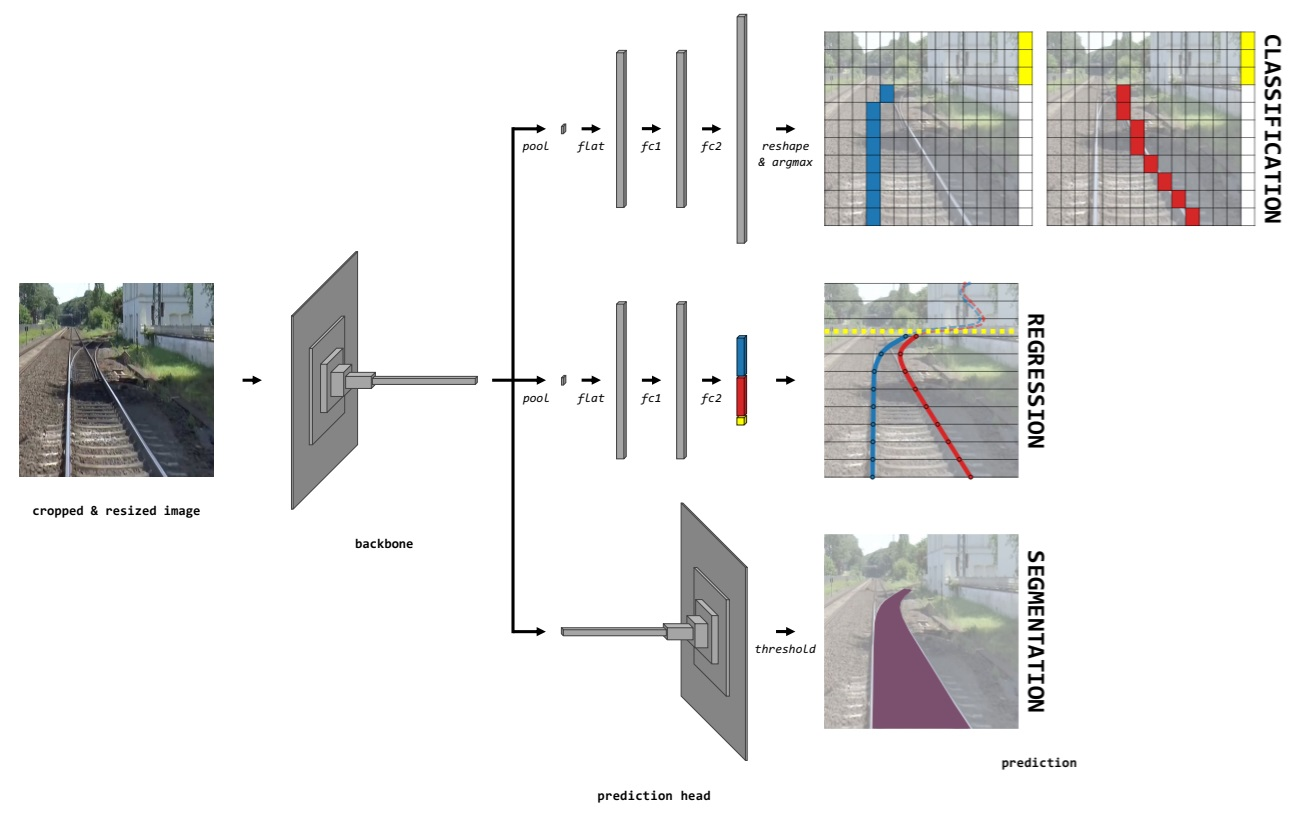
\includegraphics[width=\linewidth]{PICs/Baselinepaper/tep-net_sota_models.jpg}
    \caption{The model architecture is designed to enable a fair comparison between the novel regression model proposed in \cite{tepNet2024} and other \ac{SOTA} approaches.
    All models use the same dataset with preprocessing steps to fit annotation to the model task.}
    \label{fig:TEP-Net_sota_models}
\end{figure}

\noindent Experiments include trainings with different versions of ResNet and EfficientNet backbones.
According to the \ac{IoU}, the segmentation model is the most accurate \cite{tepNet2024}.
However, the performance difference is within a range of only 1.4 percent.
Classification with ResNet18 performs worst.
While segmentation with EfficientNet-B3 achieves the highest accuracy, it is also the slowest.
In terms of speed, the regression-based approach outperforms other models.
Additionally, it proves to be lightweight because of a lower number of parameters and \ac{MACs}.
These characteristics are of great importance for this work's rail track prediction application.
For more detailed results, please refer to \cite{tepNet2024}.

\begin{figure}[H]
    \centering
    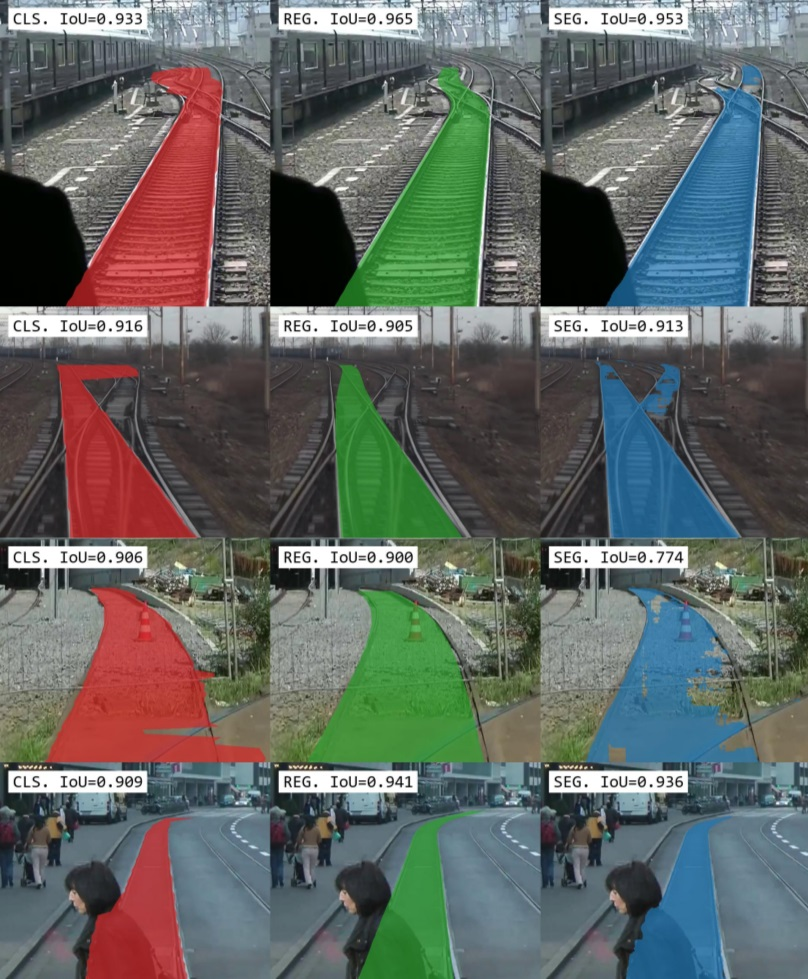
\includegraphics[width=0.7\linewidth]{PICs/Baselinepaper/comparison_sota_tep-net.jpg}
    \caption{Comparison between classification (CLS), regression (REG), and segmentation (SEG) models with challenging scenes.
    The worst backbone (ResNet18) is used for this figure to clearly show the difference in behaviors \cite{tepNet2024}.}
    \label{fig:TEP-Net_sota_comparison}
\end{figure}

\noindent Since all three model architectures achieve similar \ac{IoU} scores, \cite{tepNet2024} compares performances on individual challenging scenes.
\autoref{fig:TEP-Net_sota_comparison} visualizes a drop in accuracy when the model becomes unsure.
However, the regression model is the only one that keeps the form of a rail when the track splits and seems to have no issues with obstructions.
This is because the concept of distance in the error between prediction and \ac{GT} is only provided in the regression-based model but is missing in segmentation and classification models.
The cross-entropy loss for classification and the dice loss for segmentation both penalize misclassifications but do not account for increasing distance from the \ac{GT}.
These models work with probabilities, which tend towards extremes under certainty.
When uncertain, segmentation models move closer to a threshold, and classification models show more spread-out probabilities across classes.
The regression approach inherently involves continuous values, which assume averages among uncertain possibilities.
Resulting in a more robust system \cite{tepNet2024}.

\subsection{Limitation}
\label{sec:limitationBaseline}

The main limitation of \cite{tepNet2024} lies in its single-frame-based model architecture.
This model cannot capture temporal context, which becomes problematic when the train encounters a switch.
An example scenario is illustrated in \autoref{fig:limitationSwitch}.
Typically, the model effectively predicts the train's path when approaching switches, with all necessary information contained within the frame.
However, once the train passes over the switch and the start of the switch is no longer visible, the model cannot determine the continuation of the ego path.
Only after a certain duration does the correct track become identifiable again.

\vspace{1cm}

\begin{figure}[H]
    \centering

    % Oberes Grid mit großen Bildern
    \begin{minipage}{0.328\textwidth}
        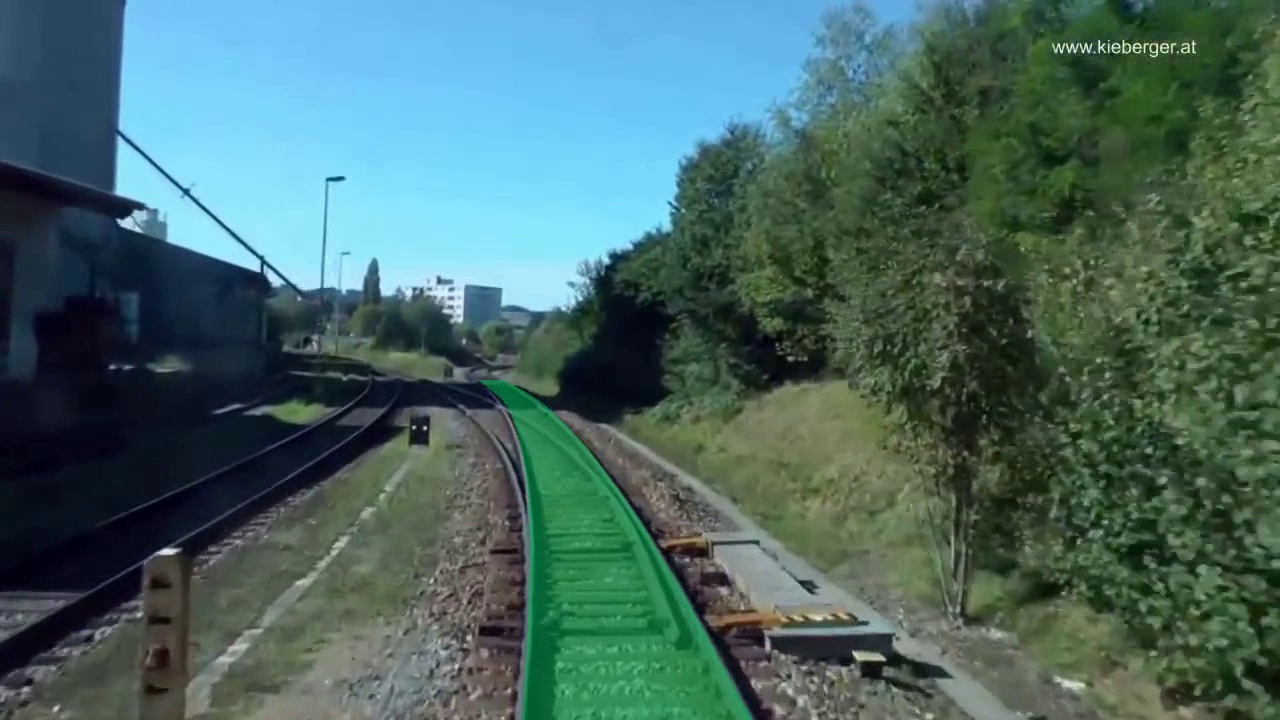
\includegraphics[width=\textwidth]{PICs/Baselinepaper/limitation_1.png}
    \end{minipage}
    \hfill
    \begin{minipage}{0.328\textwidth}
        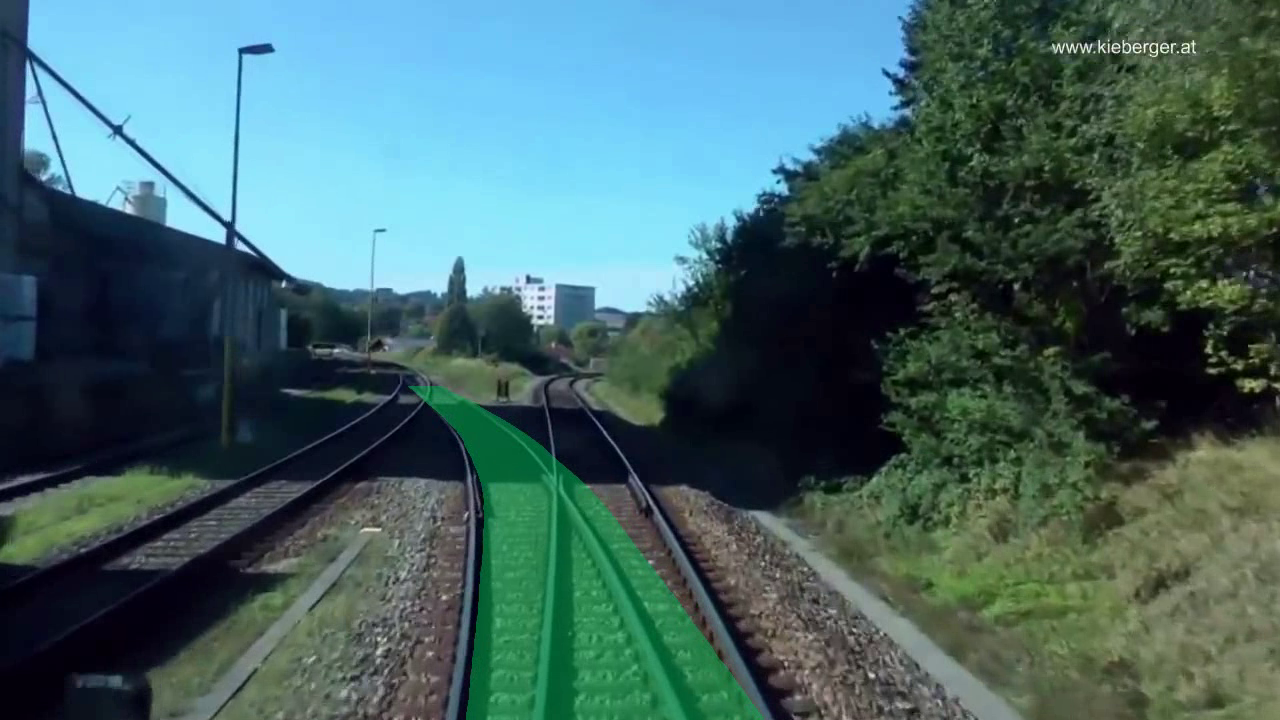
\includegraphics[width=\textwidth]{PICs/Baselinepaper/limitation_3.png}
    \end{minipage}
    \hfill
    \begin{minipage}{0.328\textwidth}
        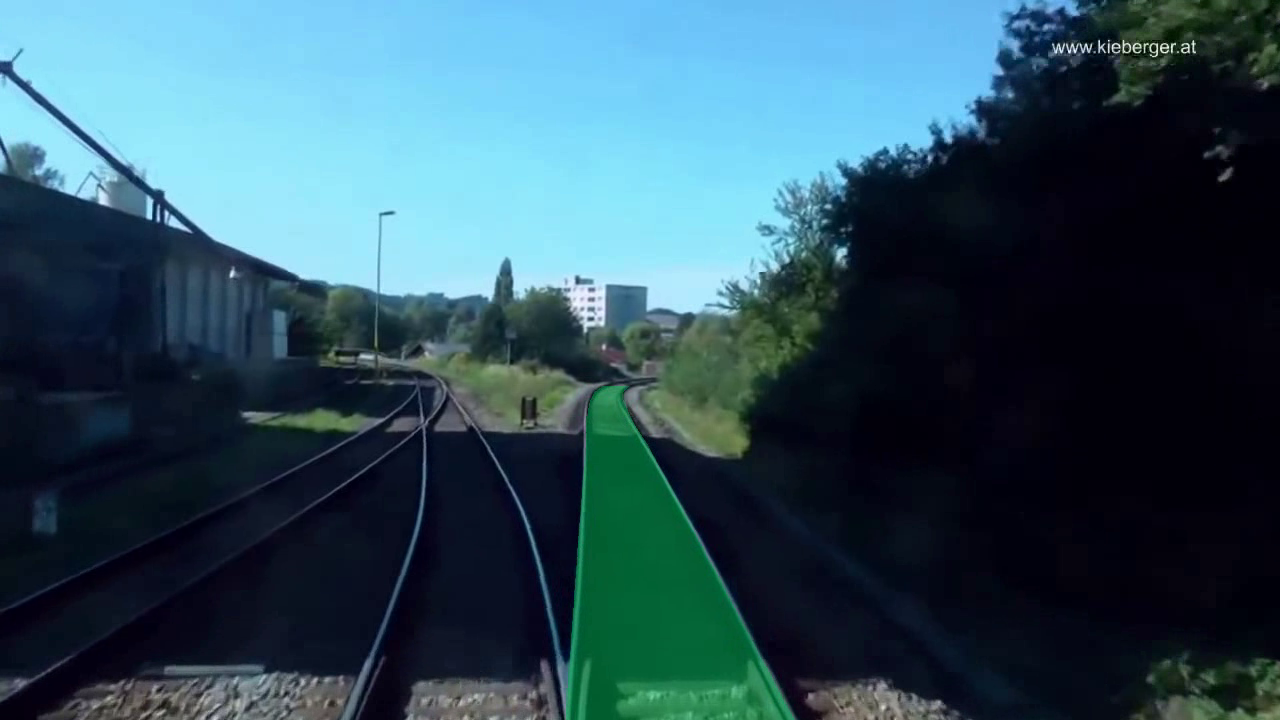
\includegraphics[width=\textwidth]{PICs/Baselinepaper/limitation_5.png}
    \end{minipage}

    \vspace{-0.15cm} % Kleinerer Abstand
    
    % Dritte Reihe nur für die Pfeile (zwischen oberen und unteren Bildern)
    \begin{minipage}{0.16\textwidth}
        \begin{tikzpicture}
            \node[anchor=south] (img) at (0,0) {};
            \draw[->, thick] (1.1,-0.1) -- (1.1,0.1); % Kürzerer Pfeil nach oben für das 1. Bild der unteren Reihe
        \end{tikzpicture}
    \end{minipage}
    \hfill
    \begin{minipage}{0.16\textwidth}
        % Kein Pfeil für dieses Bild
    \end{minipage}
    \hfill
    \begin{minipage}{0.16\textwidth}
        \begin{tikzpicture}
            \node[anchor=south] (img) at (0,0) {};
            \draw[->, thick] (0.5,-0.1) -- (0.5,0.1); % Kürzerer Pfeil nach oben für das 3. Bild der unteren Reihe
        \end{tikzpicture}
    \end{minipage}
    \hfill
    \begin{minipage}{0.16\textwidth}
        % Kein Pfeil für dieses Bild
    \end{minipage}
    \hfill
    \begin{minipage}{0.16\textwidth}
        \begin{tikzpicture}
            \node[anchor=south] (img) at (0,0) {};
            \draw[->, thick] (0.1,-0.1) -- (0.1,0.1); % Kürzerer Pfeil nach oben für das 5. Bild der unteren Reihe
        \end{tikzpicture}
    \end{minipage}
    \hfill
    \begin{minipage}{0.16\textwidth}
        % Kein Pfeil für dieses Bild
    \end{minipage}
    
    % Unteres Grid mit kleineren Bildern
    \begin{minipage}{0.16\textwidth}
        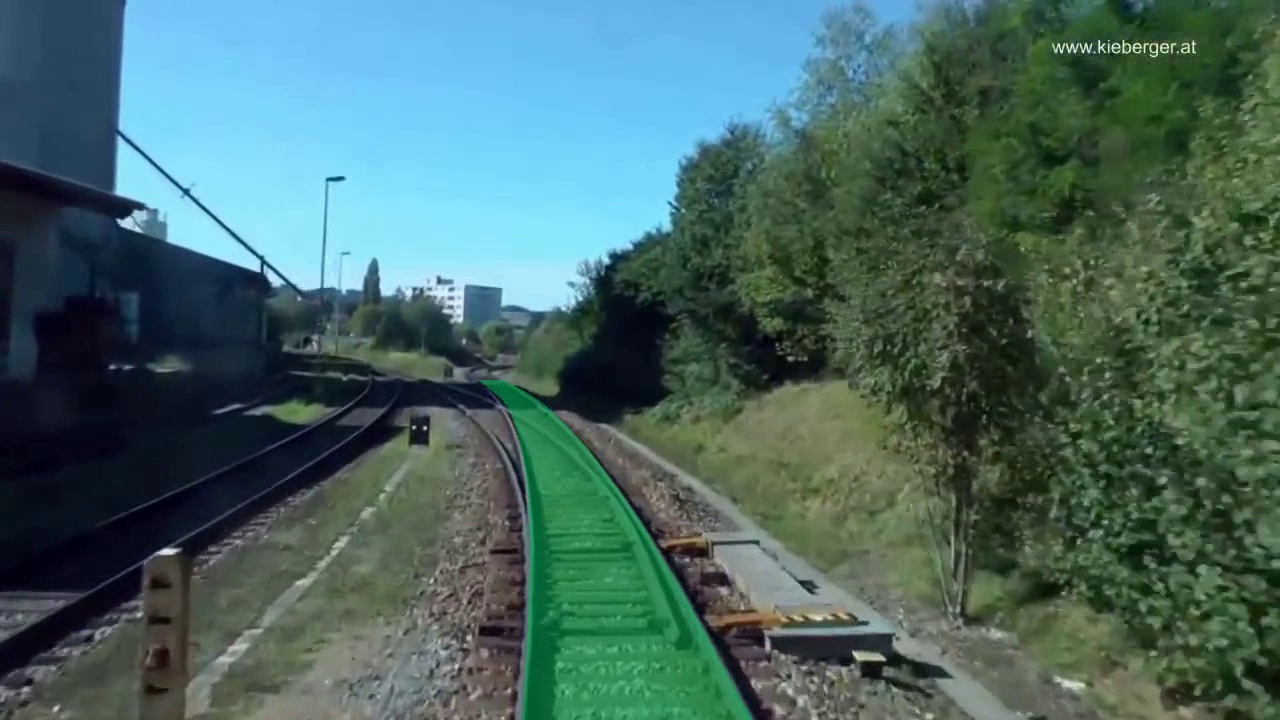
\includegraphics[width=\textwidth]{PICs/Baselinepaper/limitation_1.png}
    \end{minipage}
    \hfill
    \begin{minipage}{0.16\textwidth}
        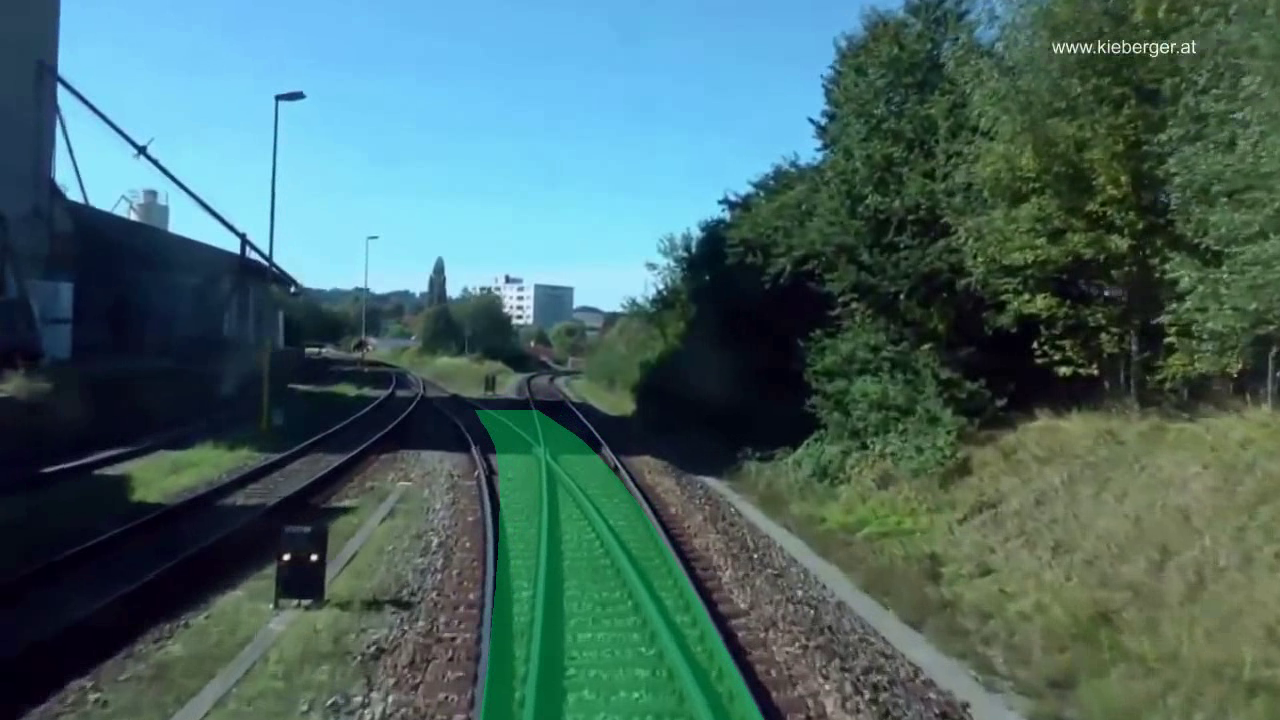
\includegraphics[width=\textwidth]{PICs/Baselinepaper/limitation_2.png}
    \end{minipage}
    \hfill
    \begin{minipage}{0.16\textwidth}
        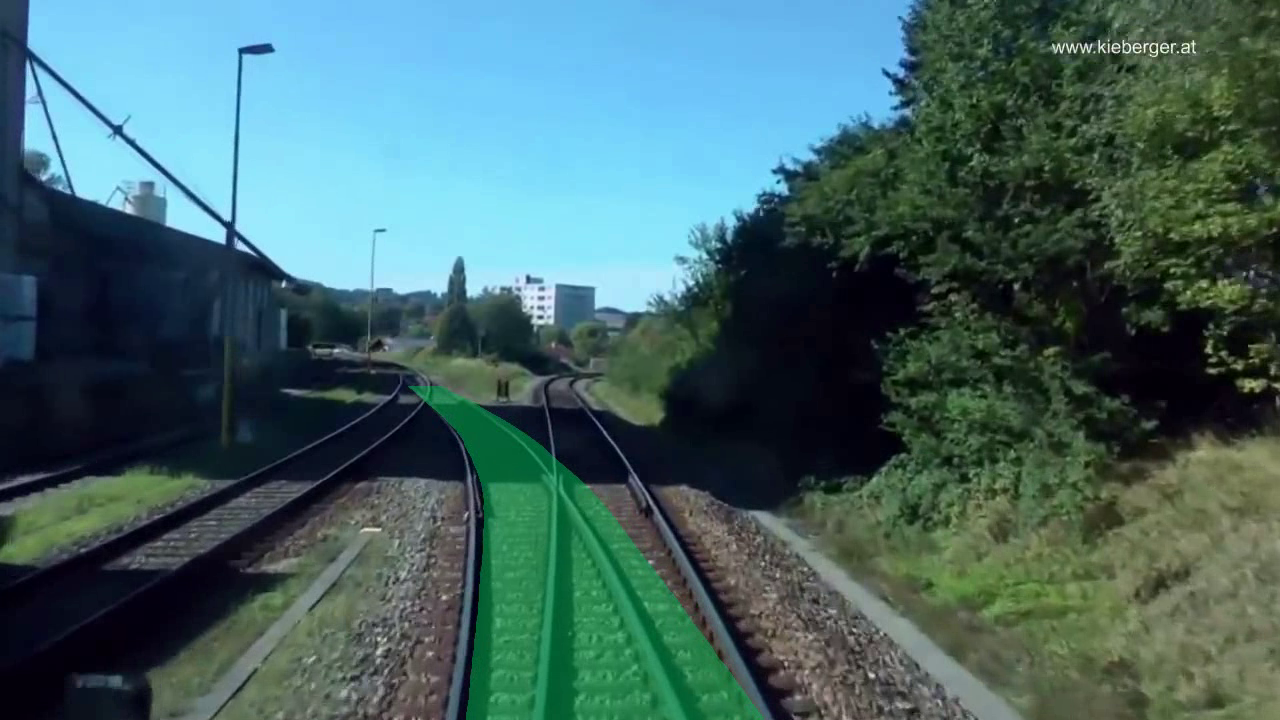
\includegraphics[width=\textwidth]{PICs/Baselinepaper/limitation_3.png}
    \end{minipage}
    \hfill
    \begin{minipage}{0.16\textwidth}
        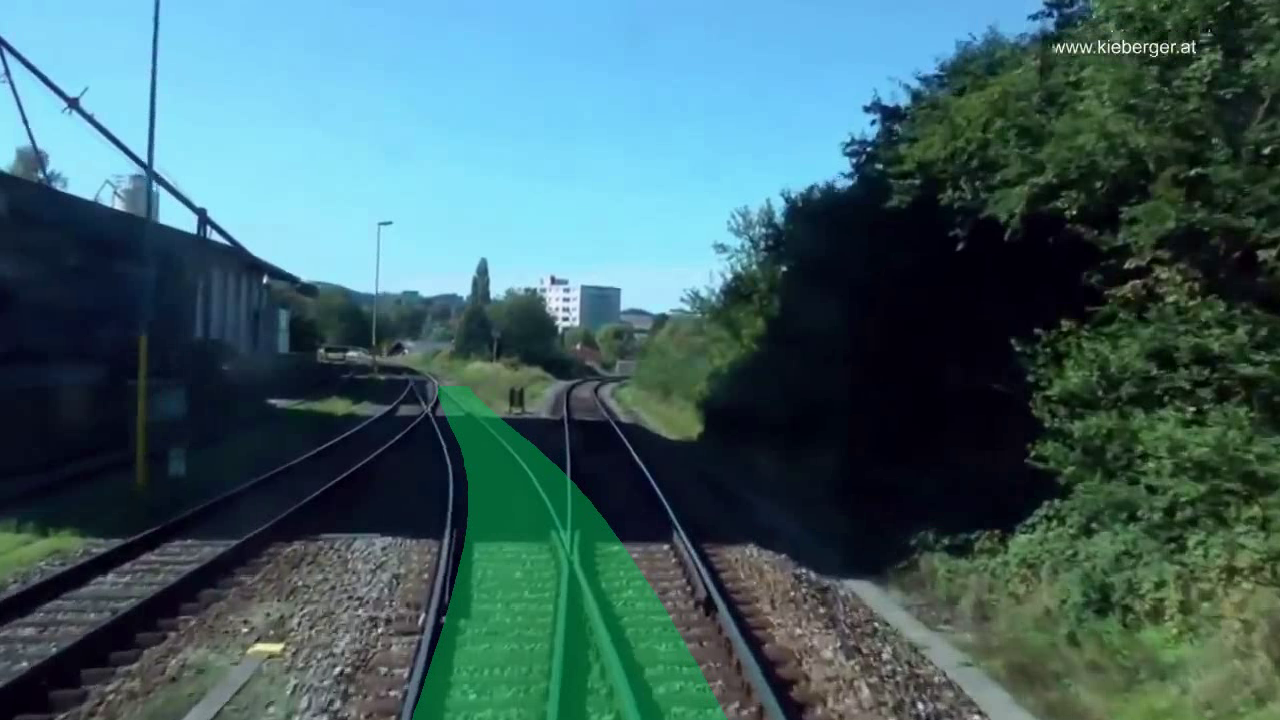
\includegraphics[width=\textwidth]{PICs/Baselinepaper/limitation_4.png}
    \end{minipage}
    \hfill
    \begin{minipage}{0.16\textwidth}
        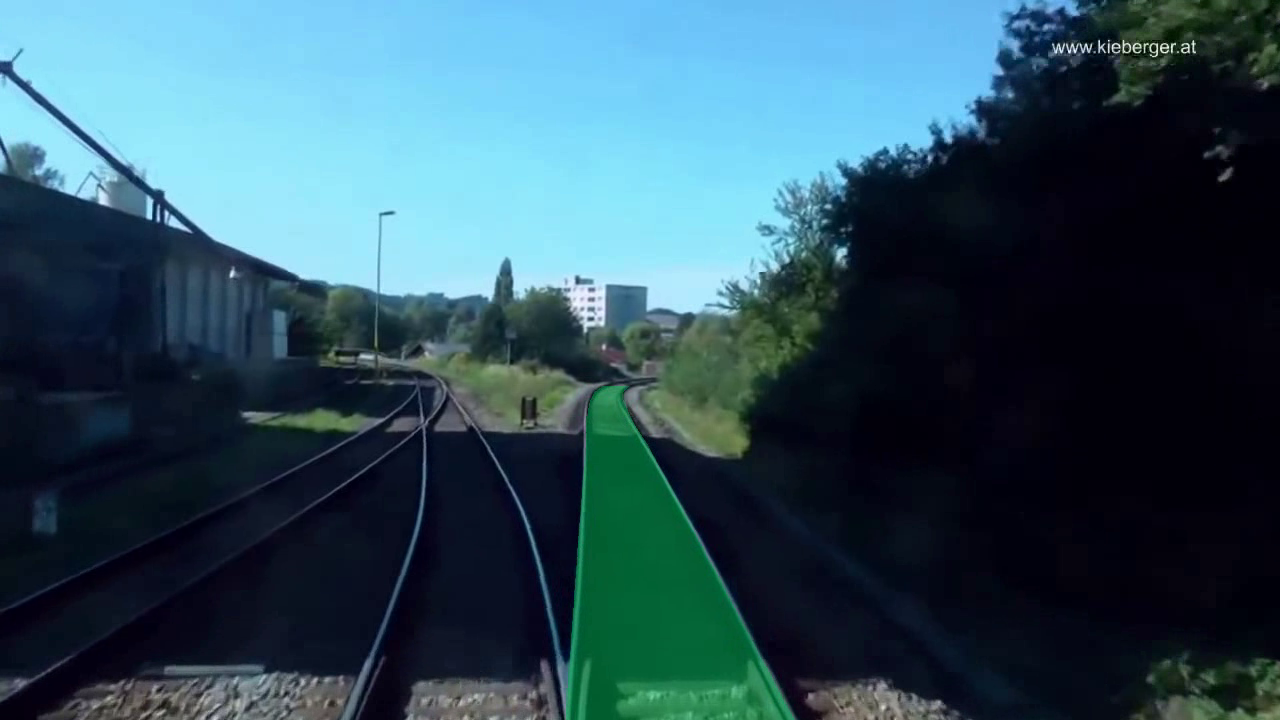
\includegraphics[width=\textwidth]{PICs/Baselinepaper/limitation_5.png}
    \end{minipage}
    \hfill
    \begin{minipage}{0.16\textwidth}
        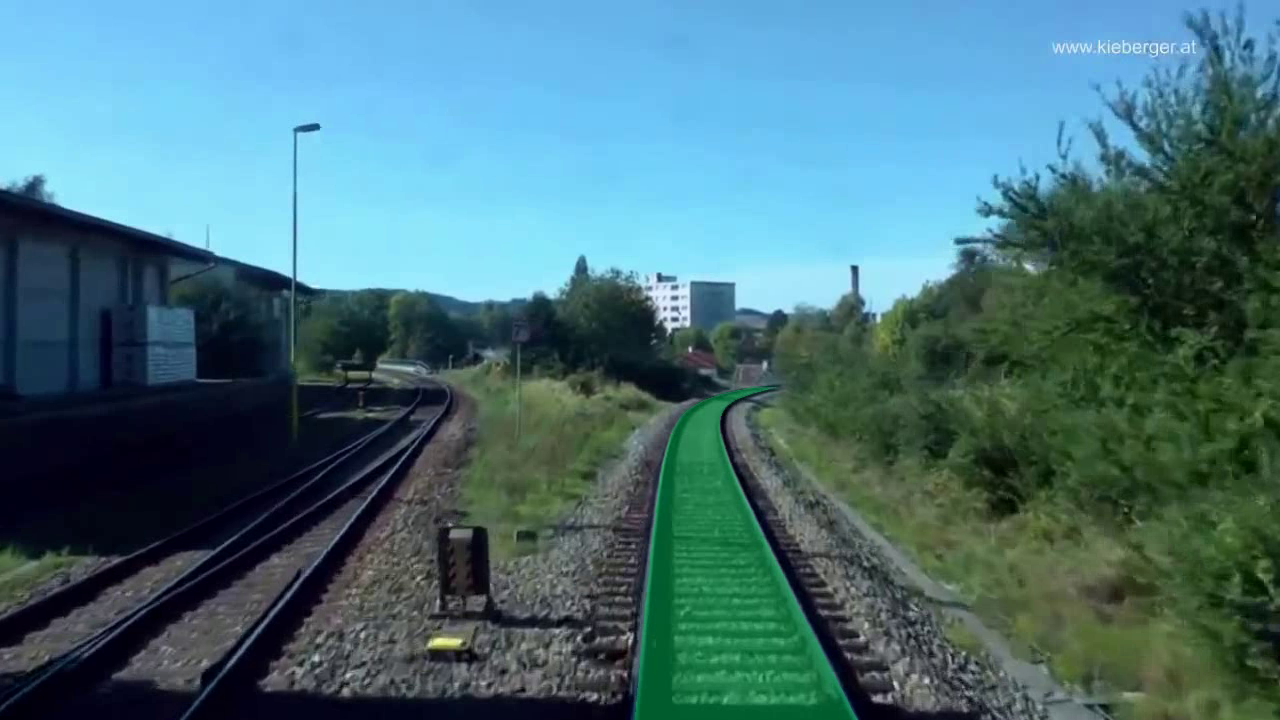
\includegraphics[width=\textwidth]{PICs/Baselinepaper/limitation_6.png}
    \end{minipage}

    % Vierte Reihe für die Zeitachse
    \begin{minipage}{1.0\textwidth}
        \centering
        \begin{tikzpicture}
            % Zeit "Time" über dem Pfeil links positionieren
            \node at (-7.5, 0.3) {time}; % Text "Time"
            \draw[-Stealth, thick] (-8, 0) -- (8, 0); % Pfeil von ganz links nach ganz rechts
        \end{tikzpicture}
    \end{minipage}

    % Beschriftung unter dem Grid
    \vspace{0.5cm}
    \caption{Limitation of \ac{TEP}-Net \cite{tepNet2024}. The introduced approach is a single-frame-based model. Therefore, no temporal context can be captured, which leads to uncertainty in prediction when driving over a switch.
    All images are from \cite{limitaion_youtube_video}. A YouTube video, which is also used by RailSem19. It is ensured that none of the frames are included in the dataset, creating a fair test scenario.}
    \label{fig:limitationSwitch}
\end{figure}

\vspace{0.5cm}

\noindent There are two approaches suggested in \cite{tepNet2024}.
The first one includes integrating a confidence score to tell if the model is in a scenario where it is prone to become unreliable.
The second suggested approach is more complete.
It would encounter the temporal component by implementing a model like a \ac{RNN}, that can capture temporal information.
However, \cite{tepNet2024} states that there is no public temporal dataset available, which fits this task.
To the best of the author's knowledge, this statement is correct.
Therefore, a corresponding dataset must also be created, if this approach is pursued.